%!TEX root = ../main.tex

In this chapter a few technical concepts will be explored in order to make the proposed method and what it aims to accomplish more clear.

\section{Augmented Reality}
As of yet, the definition of Augmented Reality that is most widely accepted is the one presented by Azuma\cite{azuma1997}. In this survey Augmented Reality (or AR for short) is defined as a software system that features a blend of real and virtual objects, the user can interact with it in real time and presents a 2D representation of a 3D world for both the real and virtual sides. A feature film that integrates real and virtual characters or objects is therefore strictly speaking not AR for example, because it's static content, the consumer cannot interact with it at all, let alone in real time.
In order to combine real and virtual objects both worlds must be aligned, in the sense that they must share a common origin for both position and rotation. If the virtual objects present in the real scene are not aligned the feasibility of the whole composition is compromised. The tracking of real world features as a guideline for alignment in the virtual world is one of the challenges in the field of AR. There are many techniques that have been used, such as sensor-based tracking, that uses dedicated hardware to feed the software application the position and rotation information it needs; vision-based tracking, in which the position and orientation origin of the virtual world are determined by images recognized by a computer vision algorithm. These images are named fiducial markers and can be an artificial black and white image, a "natural" images (points, lines, shapes and/or textures) or even 3D objects. Other approaches involving both sensors and vision algorithms have also been used, if the reader is interested in learning more about tracking, Zhou's survey\cite{zhou2008} on tracking is a good resource.
This method does not aim in any way to improve tracking for AR, current state-of-the-art methods will be used for that, but it's important to explain the concept a bit in order to settle the scope and expectations of the end result.

\section{Sensors}
Most smartphones and tablets in the market nowadays have built-in sensors to measure many things that are helpful for application developers, such as motion, orientation and other environmental conditions. The ones that are relevant for this method are the following:\newline
\textbf{Accelerometer}: This device measures proper acceleration relative to gravity. Its application in mobile development is to measure motion changes and to measure the device orientation relative to Earth's surface. It usually consists of 3 orthogonal axes. The output is given in m/s\textsuperscript{2} \newline
\textbf{Gyroscope}: A sensor that is capable of measuring the rate of rotation around a particular axis. It serves the same purpose as the accelerometer, but mobile devices usually have both for more robust measurements. The output is given in rad/s. In the method these will be used to acquire the 360 panoramic photograph, making sure that the device is within the same pitch while capturing all the images that will be stitched together to make the panorama. \newline
\textbf{Photometer}: There is a wide variability in terms of capacity of photometers across different devices, but the only measurement that is guaranteed is the ambient illuminance expressed in lx.  In the method it will be useful for detection of a noticeable change in ambient lighting, leading to a re-capture of the panorama. What exactly constitutes a noticeable change in ambient lighting will be determined through parameter tuning. \newline 
\textbf{Magnetometer}: In terms of mobile devices it serves the purpose of a compass, it measures the device's orientation with respect to the Earth's magnetic poles. In mobile development it is useful to get the heading of the device expressed in degrees.\newline
\textbf{GPS}: Measures the raw position of the device in three-dimensional Cartesian coordinates with origin on the center of the Earth. It can be used to determined where on planet Earth the device is located (Country, city, neighborhood, etc). It needs to have line of sight with no electromagnetic interference with at least 4 out of the 24 satellites in orbit that are used for GPS.

\section{Standard Illuminant}
In order to describe a color of a light source it is important to have detailed knowledge of the illuminant used. The International Commission on Illumination (CIE)  have defined a number of spectral power distributions, referred to as CIE standard illuminants, to provide reference spectra for colorimetric issues. The illuminants are denoted by a letter or a letter-number combination. Their spectral power distributions (SPD) are normalized to a value of 100 at a wavelength of 560 nm in following figures. Illuminants series A through D exist, all of them specializing on a different kind of light source. Fo this method the interesting one is series D, because it describes a sort of average light source, typically associated to daylight global illumination.\newline
D65 corresponds roughly to the average midday light in Western Europe / Northern Europe (comprising both direct sunlight and the light diffused by a clear sky), hence it is also called a daylight illuminant. It has a correlated colour temperature of approximately $6500 K$. As any standard illuminant is represented as a table of averaged spectrophotometric data, any light source which statistically has the same relative spectral power distribution (SPD) can be considered a D65 light source. It is important to note that D65 is purely theoretical, there are no actual artificial D65 light sources.\cite{DeeSixFive}

\section{Panoramic photography}
Panoramic photography is a technique of photography, using specialized equipment or software, that captures images with horizontally, and sometimes also vertically, elongated fields of view. While there is no formal definition of the minimum field of view required for a photograph to be considered panoramic, in this work the interest is focused upon those that capture the entire 360 degrees of horizontal field of view. \newline
There are different kinds of panoramic images, the most intuitive is the one called wide format photograph. It basically consists of a series of photos taken from the same height and later stitched together to appear as a single wide image. The image can be then projected on to a cylinder. This kind of panoramic photograph captures 360 degrees of horizontal field of view, while the vertical field of view is dependant entirely on the lens used to capture the individual photographs. Figure 3.1 shows an example of a cylindrical panoramic image. 

\begin{figure}[H]
  \centering
  \setlength{\unitlength}{\textwidth} 
    \begin{picture}(1,0.5)
       \put(-0.1,0){\includegraphics[width=1.3\unitlength]{Figures/pano6.jpg}}
       
    \end{picture}
    \caption{A cylindrical panorama of Trafalgar Square}
\end{figure}

The type of panoramic image used in this method is called equirectangular panoramic image, or spherical panoramic image, due to the fact that the resulting image can be projected on to a sphere. The projection maps meridians to vertical straight lines of constant spacing, and circles of latitude to horizontal straight lines of constant spacing. This kind of projection introduces the types of distortion often seen in spherical projections, such as Mercator, the poles of the sphere appear bigger than they really are. The process used by Google to create equirectangular panoramic images on mobile devices involves taking several pictures of the environment and using the device's sensors prematurely project them onto a sphere in their position relative to Earth's north. Once all pictures are captured they are stitched together in a similar manner as for cylindrical mapping, for each individual image features are identified, those same features are searched on neighboring images and aligned and the overlap is blended, resulting in a seamless, yet distorted representation of all the images as one. After this, the projection is applied as follows: \newline

\begin{equation}
    \lambda = \frac{x}{cos(\phi_l )} + \lambda_0
\end{equation}

\begin{equation}
    \phi = y + \phi_l
\end{equation}

Where: \newline
$\lambda$ is the longitude of the location to project. \newline
$\phi$ is the latitude of the location to project. \newline
$\phi_l$ are the standard parallels (north and south of the equator) where the scale of the projection is true. \newline
$\lambda_0$ is the central meridian of the map. \newline
$x$ is the horizontal coordinate of the projected location on the map. \newline
$y$ is the vertical coordinate of the projected location on the map. \newline

The kind of expected result can be seen on figure 3.2
\begin{figure}[H]
  \centering
  \setlength{\unitlength}{\textwidth} 
    \begin{picture}(0.8,0.5)
       \put(-0.1,0){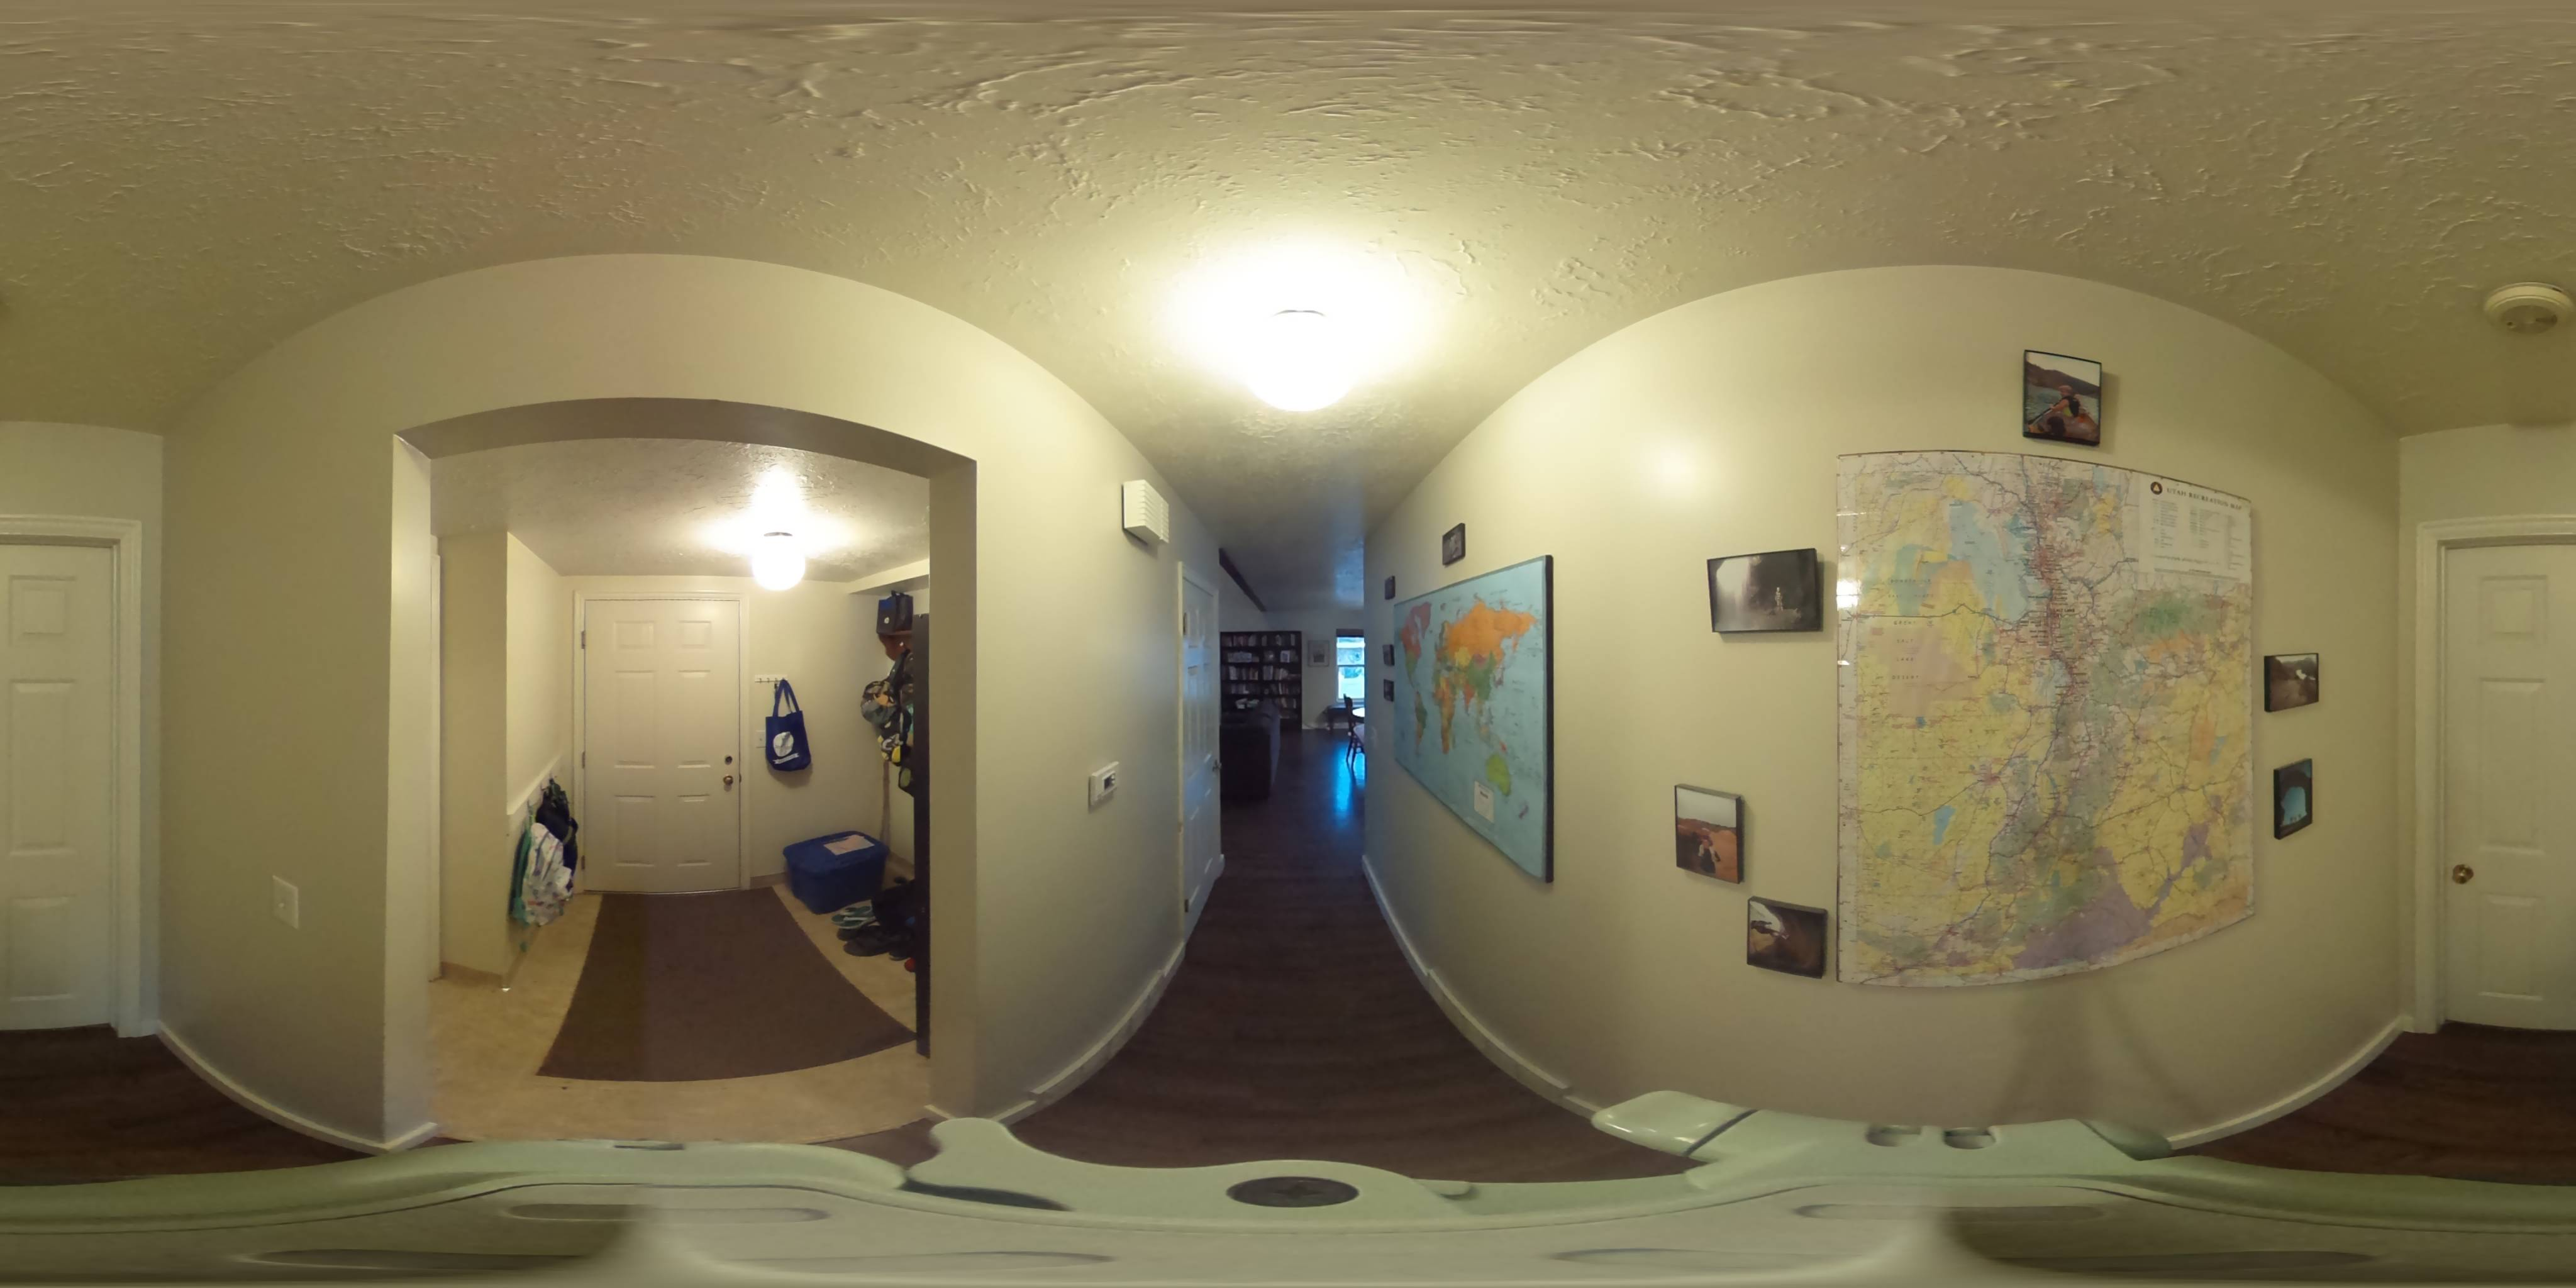
\includegraphics[width=1.0\unitlength]{Figures/equirectangular.jpg}}
       
    \end{picture}
    \caption{An average indoors equirectangular panorama}
\end{figure}